\documentclass[a4paper,11pt]{report}
\usepackage[T1]{fontenc}
\usepackage[a4paper,margin=1.5cm]{geometry}

\usepackage{amsmath}
\usepackage{amsthm}
\usepackage{booktabs}
\usepackage{graphicx}
\usepackage{stmaryrd}
\usepackage{circus}
\usepackage{listings}
\usepackage{xcolor}
% fonts
\usepackage{libertine}
\usepackage{inconsolata}

\usepackage{hyperref}
\usepackage{cleveref}

% Open question.
\newcommand{\todo}[1]{\textcolor{orange}{(#1)}}
\newcommand{\metaref}[1]{{\sffamily\slshape #1}}

\theoremstyle{definition}
\newtheorem{defn}{Definition}

\newcommand{\thead}[1]{\textbf{#1}}
\newcommand{\tsubhead}[1]{\textit{#1}}


\lstset{
	basicstyle={\small\ttfamily}	
}
\lstdefinelanguage{RoboCert}{
	morekeywords={
	anything,
	as,
	end,
	event,
	from,
	for,
	loop,
	module,
	operation,
	sequence,
	then,
	to,
	until,
	world,
	},
	morecomment=[l]{//},
	morecomment=[s]{/*}{*/},
	morestring=[b]",
}
\newcommand{\lquote}[1]{\text{`\lstinline[language=RoboCert]{#1}'}}

\newcommand{\langname}{{\sffamily\slshape RoboCert}}

\title{\langname{} Sequence Diagram Prototype}
\author{Matt Windsor}

\begin{document}
\maketitle

\tableofcontents{}

\section*{How to read this report}
%!TEX root=./robocert.tex

\emph{This manual is not yet aimed at an external audience}.

\section*{Structure}
This manual is laid out as follows:

\begin{enumerate}
\item
  Information about \langname, its purpose, and this manual;
\item
  An introduction to each notation supported by \langname, discussing the
  metamodel and any concrete notations attached to each;
\item
  The formal semantics of \langname, provided as a separate development for
  each target verification language (CSP, PRISM, etc.).
\end{enumerate}

\section*{Typography}
This report uses various typographical conventions:

\begin{itemize}
\item
	\todo{This style} represents open questions; these should be
	resolved before the report is closed.
\item
	\metaref{This style} represents metamodel names.
\item
	\texttt{This style} represents concrete textual syntax.  Boldface
	denotes keywords in the textual language.
\end{itemize}

Certain chapters may have extra conventions, which will be documented in
similar sections at the start of the corresponding chapter.

The key words \rfcmust, \rfcmustnot, \rfcrequired, \rfcshall, \rfcshallnot,
\rfcshould, \rfcshouldnot, \rfcrecommended, \rfcmay, and \rfcoptional{} in this
document are to be interpreted as described in RFC 2119.

%%% Local Variables:
%%% mode: latex
%%% TeX-master: "robocert"
%%% End:


\chapter{Abstract syntax}
%!TEX root=../robocert.tex
% Metamodel: CSP-M
\newcommand{\mcspfragment}{\metaref{CSPFragment}}
\newcommand{\meventsetcspfragment}{\metaref{EventSetCSPFragment}}
\newcommand{\minlinecspfragment}{\metaref{InlineCSPFragment}}
\newcommand{\mprocesscspfragment}{\metaref{ProcessCSPFragment}}
\newcommand{\mcsprefinementproperty}{\metaref{CSPRefinementProperty}}
\newcommand{\mcspprocesssource}{\metaref{CSPProcessSource}}
\newcommand{\mcspcontextsource}{\metaref{CSPContextSource}}


This chapter discusses the metamodel of \langname{} sequences.  This metamodel
has multiple concrete notations ---
the \emph{textual} (\cref{cha:seq-textual}) and \emph{graphical}
syntax (\cref{cha:seq-graphical}) --- and a semantics (\cref{cha:semantics-intro}). 

\section{Introduction}\label{sec:metamodel-intro}

For information on how to read the rest of this chapter, see the notes on
the top-level metamodel (\cref{ssec:core-metamodel-intro-readme}).

\subsection{A note on ordering and timing}\label{ssec:metamodel-intro-ordering}

By default, \langname{} sequences are \emph{explicit}
as to \emph{which} actions occur, but \emph{implicit} as to
\emph{when}.

Unless modified by gaps,
communications on \langname{} sequences are strictly ordered with
respect to each other and permit no intervening communications.  This
reflects the view of sequence diagrams as representations of traces of
the system under test, and appears consistent with some semantic
treatments of UML~\cite{lima-semantics}.  \todo{needs more
  justification?  is the point about Lima's semantics correct?}

Like \robochart, \langname{} has a discrete-time model, where time is
measured in \emph{time units} and events, operation calls, and
primitive data operations (assignments, communication, and so on) are
instantaneous.  Time cn pass when the software is waiting for an
interaction with the platform.  Accordingly, any amount of time may
pass in a sequence, unless constrained by \mdeadlinestep s
(\cref{ssec:metamodel-steps-deadlines}).

\section{Sequences}\label{sec:metamodel-sequences}
%!TEX root=../robocert.tex
\begin{figure}
	\centering
	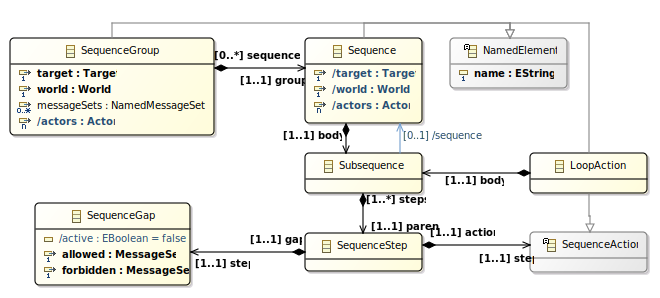
\includegraphics[width=\textwidth]{diagrams/Sequences}
	\caption{Class diagram for the part of the \langname{} metamodel dealing with sequences.}
	\label{fig:metamodel-sequences}
\end{figure}

\Cref{fig:metamodel-sequences} depicts the part of the metamodel concerning
sequence diagrams and their high-level structure.

\subsection{\msequencegroup}

A \msequencegroup{} is a top-level container for sequence diagrams.
It is a \mnamedelement{} that contains:

\begin{itemize}
\item
  two \mactor s (\cref{sec:metamodel-actors}):
  a \mtarget{} (\cref{ssec:metamodel-actors-target})
  and a \mworld{} (\cref{ssec:metamodel-actors-world});
\item
  zero or more \mnamedmessageset{}s (\cref{ssec:metamodel-messages-named-sets});
\item
  zero or more \msequence{} (\cref{ssec:metamodel-sequences-sequences}).
\end{itemize}

\begin{lstlisting}[style=Example]
sequence group Group:
  module AModule  // RCModuleTarget actor
  -> world        // World actor
{
  message set M1: universe
  
  sequence Example1 {
    anything until end
  }
  sequence Example2 {
    anything until end
  }
}
\end{lstlisting}

\subsection{\msequence}\label{ssec:metamodel-sequences-sequences}

A \msequence{} represents a sequence diagram.  It is a \mnamedelement{}
that contains a \msubsequence{} (\cref{ssec:metamodel-sequences-subsequences})
capturing the body of the diagram.

\begin{figure}[h!]

  \begin{subfigure}[t]{\egtextwidth}
    \begin{lstlisting}[style=Example]
sequence Example {
  anything until end  // Subsequence
}
    \end{lstlisting}
  \end{subfigure}
  \hfill
  \begin{subfigure}[t]{\eggraphicalwidth}
    \gsecaption
    \centering
    \begin{tikzpicture}
      \matrix[diagram]{
        \node[rcmodule](mstart) {\egtarget}; & \node[world](wstart) {\egworld}; \\
	\coordinate(mend); & \coordinate(wend); \\
      };
      \gseq{wstart}{mstart}{wend}{mend}{Example}
      \draw[lifeline] (wstart) -- (wend);
      \draw[lifeline] (mstart) -- (mend);
      \gfinal{mend}{wend}
      \ggapout{mend}{\guniverse}
    \end{tikzpicture}
  \end{subfigure}

\end{figure}

\subsection{\msubsequence}\label{ssec:metamodel-sequences-subsequences}

A \msubsequence{} is a sequential composition of one or more \msequencestep s
(\cref{ssec:metamodel-sequences-steps}).
All \msequence s contain exactly one \msubsequence{} at the top level, but
may contain multiple nested \msubsequence s introduced by constructs such as
\mloopaction s.

\begin{figure}[h!]

  \begin{subfigure}[t]{\egtextwidth}
    \begin{lstlisting}[style=Example]
{
  anything until -> operation O1()
  // ^ SequenceStep
  then -> operation O2()
  // ^ SequenceStep
  then end
  // ^ SequenceStep
}
    \end{lstlisting}
  \end{subfigure}
  \hfill
  \begin{subfigure}[t]{\eggraphicalwidth}
    \gsecaption
    \centering
    \begin{tikzpicture}
      \matrix[diagram]{
        \node[rcmodule](mstart) {\egtarget}; & \node[world](wstart) {\egworld}; \\
	\coordinate(mo1); & \coordinate(wo1); \\
	\coordinate(mo2); & \coordinate(wo2); \\
	\coordinate(mend); & \coordinate(wend); \\
      };
      \gseq{wstart}{mstart}{wend}{mend}{Example}
      \draw[lifeline] (mstart) -- (mo1) -- (mo2) -- (mend);
      \draw[lifeline] (wstart) -- (wo1) -- (wo2) -- (wend);

      \goperation{mo1}{wo1}{O1()}
      \ggapout{mo1}{\guniverse}
      \goperation{mo2}{wo2}{O2()}
      
      \gfinal{mend}{wend}

    \end{tikzpicture}
  \end{subfigure}

\end{figure}

\subsection{\msequencestep}\label{ssec:metamodel-sequences-steps}

A \msequencestep{} is a single step in a \msubsequence.  It consists of a
\msequencegap{} (\cref{ssec:metamodel-sequences-gaps}) and a
\msequenceaction{} (\cref{sec:metamodel-actions}).

\begin{lstlisting}[style=Example]
anything until -> operation O()
// SequenceStep with explicit SequenceGap and SequenceAction

-> operation O()
// SequenceStep with explicit SequenceAction only;
// implicit SequenceGap with empty allow set
\end{lstlisting}

\subsection{\msequencegap}\label{ssec:metamodel-sequences-gaps}

A \msequencegap{} represents a condition on any
communication\footnote{In PSCs, this would correspond to
  \emph{intraMSG}s.} that can happen \emph{before} a \msequenceaction.
It contains two \mmessageset s (\cref{ssec:metamodel-messages-sets}):
one specifying the messages \emph{allowed} to pass inside the gap, and
another specifying the messages \emph{forbidden} to pass.

\begin{figure}[h!]

  \begin{subfigure}[c]{\egtextwidth}
    \begin{lstlisting}[style=Example]
anything
in message set MS
except {| -> operation O2() |}
until

anything in message set MS until
// implicit 'except {||}'

anything until
// implicit 'in universe {||}'
\end{lstlisting}
  \end{subfigure}
  \hfill
  \begin{subfigure}[c]{\eggraphicalwidth}
    \gsecaption
    \centering
    \begin{tikzpicture}
      \matrix[diagram, column sep=15em]{
        \coordinate(m1); & \coordinate(w1); \\
        \coordinate(m2); & \coordinate(w2); \\
        \coordinate(m3); & \coordinate(w3); \\
      };
      \draw[dotted] (m1) -- (w1);
      \ggapout{m1}{\gdiff{\grefset{MS}}\gextset{\text{\lstinline[language=RoboCert]{-> operation O2()}}}}
      
      \draw[dotted] (m2) -- (w2);
      \ggapin{w2}{\grefset{MS}}
      
      \draw[dotted] (m3) -- (w3);
      \ggapout{m3}{\guniverse}
    \end{tikzpicture}
  \end{subfigure}

\end{figure}

%%% Local Variables:
%%% mode: latex
%%% TeX-master: "../robocert"
%%% End:


\section{Steps}\label{sec:metamodel-steps}
%!TEX root=../robocert.tex
\begin{figure}[htb]
	\centering
	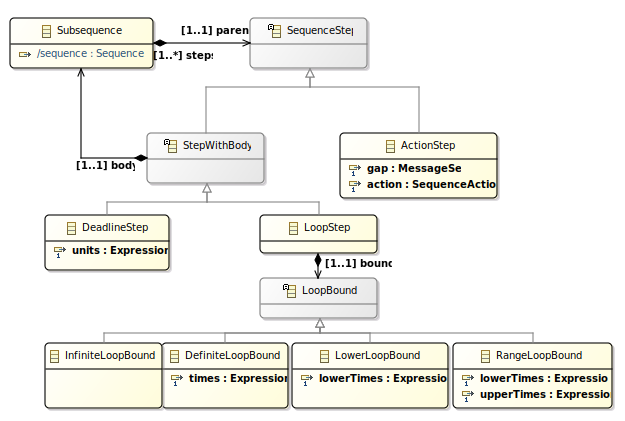
\includegraphics[width=0.7\textwidth]{diagrams/Steps}
	\caption{Class diagram for the part of the \langname{} metamodel dealing with steps.}
	\label{fig:metamodel-steps}
\end{figure}

\noindent
Steps (\msequencestep) are elements of
\msubsequence s.  They represent both communications and control flow, and
can themselves contain \msubsequence s.  There are three types of
step:

\begin{itemize}
\item \mdeadlinestep{} (\cref{ssec:metamodel-steps-deadlines});
\item \mloopstep{} (\cref{ssec:metamodel-steps-loops});
\item \mactionstep{} (\cref{ssec:metamodel-steps-actions});
\end{itemize}

\Cref{fig:metamodel-actions} depicts the part of the metamodel concerning
sequence steps.

\subsection{\mdeadlinestep}\label{ssec:metamodel-steps-deadlines}

A \mdeadlinestep{} asserts that a \msubsequence{} takes at most
a given number of time units to complete.
It takes a name (currently only
used in the graphical notation), and an expression that must
evaluate to a natural number of time units.

\begin{remark}
To specify that all actions in a \msubsequence{} must occur
immediately, use a deadline of \(0\).
\end{remark}

\begin{figure}[H]
\begin{subfigure}[t]{\egtextwidth}
\begin{lstlisting}[style=Example]
deadline T : within 3 units {
    ->op O1()
}
\end{lstlisting}
\end{subfigure}
\hfill
\begin{subfigure}[t]{\eggraphicalwidth}
  \gsecaption
  \centering
  \begin{tikzpicture}
\matrix[diagram]{
  \node[rcmodule](mstart) {\egtarget}; & \node[world](wstart) {\egworld}; \\
  & \coordinate(wds); & \\
  \coordinate(mo); & \coordinate(wo); & \\
  \coordinate(mde); & \coordinate(wde); \\
};
\draw[lifeline] (mstart) -- (mo) -- (mde);
\draw[lifeline] (wstart) -- (wds) -- (wo) -- (wde);
\gdeadline{wds}{wde}{T}{3}
\draw (mo) edge[oarrow, "O1()"] (wo);
  \end{tikzpicture}
\end{subfigure}
\end{figure}

\todo{Considering removing `deadline T :` and changing the graphical
  syntax to just contain the number of units next to the arrow, which
  I've seen rarely in some UML2 tutorials but I'm not sure if it's
  allowed in MARTE.}

\subsection{\mloopstep}\label{ssec:metamodel-steps-loops}

% Shorthand for introducing the loop action diagram matrix.
\newcommand{\egloopmatrix}{
  \node[rcmodule](mstart) {\egtarget}; \pgfmatrixnextcell \node[world](wstart) {\egworld}; \\
  \coordinate(mls); \pgfmatrixnextcell \coordinate(wls); \\
  \coordinate(mo); \pgfmatrixnextcell \coordinate(wo); \\
  \coordinate(mle); \pgfmatrixnextcell \coordinate(wle); \\
}
% Draws the entire loop diagram with the given loop bound header.
\newcommand{\egloopdiagram}[1]{
  \matrix[diagram]{\egloopmatrix};
  \draw[lifeline] (mstart) -- (mls) -- (mo) -- (mle);
  \draw[lifeline] (wstart) -- (wls) -- (wo) -- (wle);
  \draw (mo) edge[oarrow, "O1()"] (wo);
  \gloop{mls}{wls}{mle}{wle}{L}{#1}
}

A \mloopstep{} is a named loop over a \msubsequence{} of steps.
The number of times a \mloopstep{} will iterate \todo{adding breaks will
change this}
depends on its attached \mloopbound{}.  Each bound is in terms of
\mexpression{}s that are evaluated \emph{only once}, before the execution
of the loop.

\paragraph{\minfiniteloopbound}
A \minfiniteloopbound{} states that the loop executes an infinite
number of times.

\begin{figure}[H]
\begin{subfigure}[t]{\egtextwidth}
\begin{lstlisting}[style=Example]
loop L : forever { // or 'loop L {'
    ->op O1()
}
\end{lstlisting}
\end{subfigure}
\hfill
\begin{subfigure}[t]{\eggraphicalwidth}
  \gsecaption
  \centering
  \begin{tikzpicture}
    \egloopdiagram{\gloopinfinite}
  \end{tikzpicture}
\end{subfigure}
\end{figure}

\paragraph{\mdefiniteloopbound}
A \mdefiniteloopbound{} states that the loop executes exactly the
number of times given in the bound.

\begin{figure}[H]
\begin{subfigure}[t]{\egtextwidth}
\begin{lstlisting}[style=Example]
loop L : exactly 4 times {
    ->op O1()
}
\end{lstlisting}
\end{subfigure}
\hfill
\begin{subfigure}[t]{\eggraphicalwidth}
  \gsecaption
  \centering
  \begin{tikzpicture}
    \egloopdiagram{\gloopdefinite{4}}
  \end{tikzpicture}
\end{subfigure}
\end{figure}

\paragraph{\mlowerloopbound}
A \mlowerloopbound{} states that the loop executes at least the
number of times given in the bound, but may nondeterministically
choose to execute any number of times in addition.

\begin{figure}[h!]
\begin{subfigure}[t]{\egtextwidth}
\begin{lstlisting}[style=Example]
loop L : at least 5 times {
    ->op O1()
}
\end{lstlisting}
\end{subfigure}
\hfill
\begin{subfigure}[t]{\eggraphicalwidth}
  \gsecaption
  \centering
  \begin{tikzpicture}
    \egloopdiagram{\glooplower{5}}
  \end{tikzpicture}
\end{subfigure}
\end{figure}

\paragraph{\mrangeloopbound}
A \mrangeloopbound{} behaves as a \mlowerloopbound, but states that
the loop will not execute any more times than the given upper bound.
Note that if the bounds are the same, the semantics is equivalent
to that of a \mdefiniteloopbound{}.

\begin{figure}[H]
\begin{subfigure}[t]{\egtextwidth}
\begin{lstlisting}[style=Example]
loop L : between 3 and 6 times {
    ->op O1()
}
\end{lstlisting}
\end{subfigure}
\hfill
\begin{subfigure}[t]{\eggraphicalwidth}
  \gsecaption
  \centering
  \begin{tikzpicture}
    \egloopdiagram{\glooprange{3}{6}}
  \end{tikzpicture}
\end{subfigure}
\end{figure}

\subsection{\mactionstep}\label{ssec:metamodel-steps-actions}

A \mactionstep{} contains a specification of a
\msequenceaction{} (\cref{sec:metamodel-actions}), as well as
a \mmessageset{}
capturing any communications implicitly allowed to happen
in the \emph{gap} before the action.

\begin{figure}[H]
  \begin{subfigure}[c]{\egtextwidth}
    \begin{lstlisting}[style=Example]
      anything in set MS except ->op O2() until ->event E

      anything except ->op O2() until <-event E
      // shorthand for 'in {||} except ->op O2()'

      anything until ->event E
      // shorthand for 'in universe'
    \end{lstlisting}
  \end{subfigure}
  \hfill
  \begin{subfigure}[c]{\eggraphicalwidth}
    \gsecaption
    \centering
    \begin{tikzpicture}
      \matrix[diagram, column sep=15em]{
        \coordinate(m1); & \coordinate(w1); \\
        \coordinate(m2); & \coordinate(w2); \\
        \coordinate(m3); & \coordinate(w3); \\
      };
      \draw[dotted] (m1) -- (w1);
      \ggapout{m1}{\gdiff{\grefset{MS}}\gextset{\text{\lstinline[language=RoboCert]{->op O2()}}}}
      
      \draw[dotted] (m2) -- (w2);
      \ggapin{w2}{\gdiff{\guniverse}\gextset{\text{\lstinline[language=RoboCert]{->op O2()}}}}
      
      \draw[dotted] (m3) -- (w3);
      \ggapout{m3}{\guniverse}
    \end{tikzpicture}
  \end{subfigure}
\end{figure}
%%% Local Variables:
%%% mode: latex
%%% TeX-master: "../robocert"
%%% End:


\section{Actions}\label{sec:metamodel-actions}
%!TEX root=../robocert.tex
\begin{figure}
	\centering
	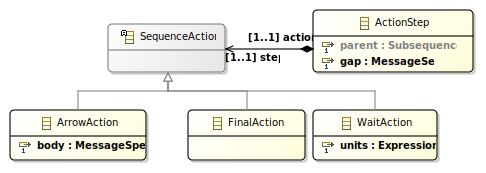
\includegraphics[width=0.7\textwidth]{diagrams/Actions}
	\caption{Class diagram for the part of the \langname{} metamodel dealing with actions.}
	\label{fig:metamodel-actions}
\end{figure}

\Cref{fig:metamodel-actions} depicts the part of the metamodel concerning
sequence actions.

A \msequenceaction{} is an explicit communication or control flow construct in a
\msubsequence.  There are currently three types of action: arrow, loop, and
final actions.

\subsection{\marrowaction}

An \marrowaction\footnote{The name signifies both that the actions resemble
PSC \emph{arrowMSG} specifications, and also that they correspond to arrows in
the graphical syntax.} specifies one communication between \mactor s which is on
the sequence specified by the diagram.  Each \marrowaction{} wraps one
\marrowmessagespec{} (\cref{sec:metamodel-messages})
containing the specification proper.
\todo{Eventually these will bind arguments.}

\begin{figure}[h!]
\begin{subfigure}[t]{\egtextwidth}
\begin{lstlisting}[style=Example]
-> operation O1()
\end{lstlisting}
\end{subfigure}
\hfill
\begin{subfigure}[t]{\eggraphicalwidth}
\gsecaption
\centering
\begin{tikzpicture}
\matrix[diagram]{
    \node[rcmodule](mstart) {\egtarget}; & \node[world](wstart) {\egworld}; \\
	\coordinate(mo); & \coordinate(wo); \\
	\coordinate(mend); & \coordinate(wend); \\
};
\draw[lifeline] (mstart) -- (mo) -- (mend);
\draw[lifeline] (wstart) -- (wo) -- (wend);
\draw (mo) edge[oarrow, "O1()"] (wo);
\end{tikzpicture}
\end{subfigure}

\end{figure}

\subsection{\mloopaction}

% Shorthand for introducing the loop action diagram matrix.
\newcommand{\egloopmatrix}{
  \node[rcmodule](mstart) {\egtarget}; \pgfmatrixnextcell \node[world](wstart) {\egworld}; \\
  \coordinate(mls); \pgfmatrixnextcell \coordinate(wls); \\
  \coordinate(mo); \pgfmatrixnextcell \coordinate(wo); \\
  \coordinate(mle); \pgfmatrixnextcell \coordinate(wle); \\
}
% Draws the entire loop diagram with the given loop bound header.
\newcommand{\egloopdiagram}[1]{
  \matrix[diagram]{\egloopmatrix};
  \draw[lifeline] (mstart) -- (mls) -- (mo) -- (mle);
  \draw[lifeline] (wstart) -- (wls) -- (wo) -- (wle);
  \draw (mo) edge[oarrow, "O1()"] (wo);
  \gloop{mls}{wls}{mle}{wle}{L}{#1}
}

A \mloopaction{} is a \emph{named} loop.  Each \mloopaction{} contains one
\msubsequence{} of steps to repeat indefinitely.

The number of times a \mloopaction{} will iterate \todo{breaking forthcoming}
depends on its attached \mloopbound{}.  Each bound is in terms of
\mexpression{}s that are evaluated \emph{only once}, before the execution
of the loop.

\paragraph{\minfiniteloopbound}
A \minfiniteloopbound{} states that the loop executes an infinite
number of times.

\begin{figure}[h!]
\begin{subfigure}[t]{\egtextwidth}
\begin{lstlisting}[style=Example]
loop L : forever { // or 'loop L {'
    -> operation O1()
}
\end{lstlisting}
\end{subfigure}
\hfill
\begin{subfigure}[t]{\eggraphicalwidth}
  \gsecaption
  \centering
  \begin{tikzpicture}
    \egloopdiagram{\gloopinfinite}
  \end{tikzpicture}
\end{subfigure}
\end{figure}

\paragraph{\mdefiniteloopbound}
A \mdefiniteloopbound{} states that the loop executes exactly the
number of times given in the bound.

\begin{figure}[h!]
\begin{subfigure}[t]{\egtextwidth}
\begin{lstlisting}[style=Example]
loop L : exactly 4 times {
    -> operation O1()
}
\end{lstlisting}
\end{subfigure}
\hfill
\begin{subfigure}[t]{\eggraphicalwidth}
  \gsecaption
  \centering
  \begin{tikzpicture}
    \egloopdiagram{\gloopdefinite{4}}
  \end{tikzpicture}
\end{subfigure}
\end{figure}

\paragraph{\mlowerloopbound}
A \mlowerloopbound{} states that the loop executes at least the
number of times given in the bound, but may nondeterministically
choose to execute any number of times in addition.

\begin{figure}[h!]
\begin{subfigure}[t]{\egtextwidth}
\begin{lstlisting}[style=Example]
loop L : at least 5 times {
    -> operation O1()
}
\end{lstlisting}
\end{subfigure}
\hfill
\begin{subfigure}[t]{\eggraphicalwidth}
  \gsecaption
  \centering
  \begin{tikzpicture}
    \egloopdiagram{\glooplower{5}}
  \end{tikzpicture}
\end{subfigure}
\end{figure}

\paragraph{\mrangeloopbound}
A \mrangeloopbound{} behaves as a \mlowerloopbound, but states that
the loop will not execute any more times than the given upper bound.
Note that if the bounds are the same, the semantics is equivalent
to that of a \mdefiniteloopbound{}.

\begin{figure}[h!]
\begin{subfigure}[t]{\egtextwidth}
\begin{lstlisting}[style=Example]
loop L : between 3 and 6 times {
    -> operation O1()
}
\end{lstlisting}
\end{subfigure}
\hfill
\begin{subfigure}[t]{\eggraphicalwidth}
  \gsecaption
  \centering
  \begin{tikzpicture}
    \egloopdiagram{\glooprange{3}{6}}
  \end{tikzpicture}
\end{subfigure}
\end{figure}

\subsection{\mfinalaction}

A \mfinalaction{} captures the successful termination of a sequence diagram.
A diagram with a \mfinalaction{} specifies a complete sequence of behaviour
from the \mtarget{} initialising to the \mtarget{} terminating.  Conversely,
sequence diagrams without \mfinalaction s capture partial specifications of
behaviour, or the behaviour of \mtarget s that do not terminate.

Note that the final \msequencegap{} before a \mfinalaction{} captures
any permitted communications after the behaviour explicitly specified by the
diagram has occurred.

\begin{figure}[h]

\begin{subfigure}[t]{\egtextwidth}
\begin{lstlisting}[style=Example]
end
\end{lstlisting}
\end{subfigure}
\hfill
\begin{subfigure}[t]{\eggraphicalwidth}
\gsecaption
\centering
\begin{tikzpicture}
\matrix[diagram]{
	\node[rcmodule](mstart) {\egtarget}; & \node[world](wstart) {\egworld}; \\
	\coordinate(mend); & \coordinate(wend); \\
};
\draw[lifeline] (mstart) -- (mend);
\draw[lifeline] (wstart) -- (wend);
\gfinal{mend}{wend}
\end{tikzpicture}
\end{subfigure}

\end{figure}

%%% Local Variables:
%%% mode: latex
%%% TeX-master: "../robocert"
%%% End:


\section{Messages}\label{sec:metamodel-messages}
%!TEX root=../robocert.tex
\begin{figure}
	\centering
	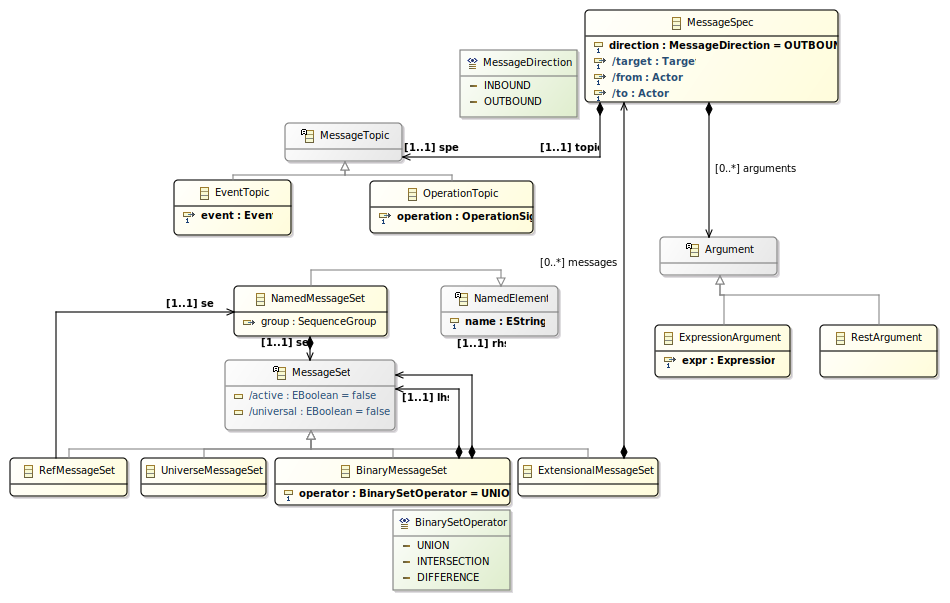
\includegraphics[width=\textwidth]{diagrams/Messages}
	\caption{Class diagram for the part of the \langname{} metamodel dealing with messages.}
	\label{fig:metamodel-messages}
\end{figure}

\Cref{fig:metamodel-messages} depicts the part of the metamodel concerning
messages between actors.  Messages are introduced into a sequence diagram
in \mmessageset s and \marrowaction s.

\subsection{\mmessageset}\label{ssec:metamodel-messages-sets}

A \mmessageset{} is an expression of the set of messages allowed or forbidden
inside a \msequencegap.  There are two types of \mmessageset:

\begin{itemize}
\item
  a \muniversemessageset{} represents the universal set containing 
  all possible messages, and
  captures a lack of specific restriction on
  the \emph{allowed} set of a \msequencegap;
\item	
  an \mextensionalmessageset{} is a set (expressed as an unordered list) of
  zero or more \mgapmessagespec s, themselves
  a type of \mmessagespec{} (\cref{sec:metamodel-messages});
\item
  a \mrefmessageset{} refers to a \mnamedmessageset{} attached to the
  sequence.
\end{itemize}

There is not yet any meaningful extra data stored in
\mgapmessagespec s that is not present in \mmessagespec s, but this is subject
to change.

\begin{lstlisting}[style=Example]
universe                 // UniverseMessageSet
{| -> operation O1() |}  // ExtensionalMessageSet
message set S            // RefMessageSet
\end{lstlisting}

\subsection{\mnamedmessageset}\label{ssec:metamodel-messages-named-sets}

A \mnamedmessageset{} attaches a name to a \mmessageset, so that it can be reused
inside a \msequence.

\begin{lstlisting}[style=Example]
message set S: {| -> operation O1() |}
\end{lstlisting}

\subsection{\mmessagespec}

A \mmessagespec{} is a specification on the types of communication that can
happen during a gap (a \mgapmessagespec) or arrow (an \marrowmessagespec).\footnote{
This class distinction resembles that in PSCs betweeen intraMSGs and arrowMSGs,
respectively.}  Each \mmessagespec{} contains:

\begin{itemize}
\item
  a \mmessagedirection; \emph{outbound} from \mtarget{} to \mworld,
  or \emph{inbound} from \mworld to \mtarget;
\item
  the \mmessagetopic{} (\cref{ssec:metamodel-messages-topics}) specifying
  the type of communication that the spec is capturing.
\end{itemize}

It is possible to infer the \mtarget{} and \mworld{} related by a
\mmessagespec{} through its containing \msequencegroup.  From these
and the \mmessagedirection, we can further infer the source (`from')
and destination (`to') \mactor s.  The target, from, and to actors are
available in EMF as derived references.

\begin{figure}[h!]

\begin{subfigure}[t]{\egtextwidth}
\begin{lstlisting}[style=Example]
-> operation O1()
// outbound MessageSpec with OperationTopic

<- event E
// inbound MessageSpec with EventTopic
\end{lstlisting}
\end{subfigure}
\hfill
\begin{subfigure}[t]{\eggraphicalwidth}
\gsecaption
\centering
\begin{tikzpicture}
\matrix[diagram]{
    \node[rcmodule](mstart) {\egtarget}; & \node[world](wstart) {\egworld}; \\
	\coordinate(mo); & \coordinate(wo); \\
	\coordinate(me); & \coordinate(we); \\
	\coordinate(mend); & \coordinate(wend); \\
};
\draw[lifeline] (wstart) -- (wo) -- (we) -- (wend);
\draw[lifeline] (mstart) -- (mo) -- (me) -- (mend);
\draw (mo) edge[oarrow, "O1()"] (wo);
\draw (we) edge[earrow, "E"'] (me);
\end{tikzpicture}
\end{subfigure}

\end{figure}

\subsection{\mmessagetopic}\label{ssec:metamodel-messages-topics}

A \mmessagetopic{} identifies the specific type of communication in a
\mmessagespec{}.  There are currently two types of topic, corresponding to
\robochart{} operations (\moperationtopic) and events (\meventtopic)
\todo{variable topics will arrive later on; \ghissue{24}}.
Each contains a reference to the signature of the respective construct.

\begin{lstlisting}[style=Example]
operation O1() // OperationTopic
event E        // EventTopic
\end{lstlisting}

\subsection{\margument}\label{ssec:metamodel-messages-arguments}

An \margument{} is a pattern that specifies (and possibly binds) one or more
arguments in
a message.  There are two types of argument:

\begin{itemize}
\item
  \mexpressionargument, which specifies that the argument is equal to the
  value of a particular \robochart{} expression;
  \todo{the \langname{} CSP generator doesn't yet properly protect against this being
    an expression not expressible as a prefix}
\item
  \mrestargument, which matches \emph{all} following arguments and permits
  them to be any value.
  \todo{This mainly exists because it's very easy to specify in CSP.  Ideally
    we'll have something that allows wildcards on arbitrary parameters, in
    which case this might be confusing to have also.}
\end{itemize}

\margument s that introduce bindings \todo{which do not exist
  yet \todo{\ghissue{12}}} may only appear in \marrowmessagespec s.
This is because bindings are only visible during the main body of a
sequence.
Consequently, any arguments that appear in
\mgapmessagespec s must be subclasses of \mnonbindingargument.

must not introduce bindings, as
any bindings that could be introduced would not 
and
this is represented by the 

All \margument s, at time of writing, are forms of \mnonbindingargument{} and
can therefore appear in \mgapmessagespec s.  This will change when binding
arguments are introduced
\todo{\ghissue{12}}.

\begin{lstlisting}[style=Example]
42  // ExpressionArgument containing integer literal
... // RestArgument
\end{lstlisting}

%%% Local Variables:
%%% mode: latex
%%% TeX-master: "../robocert"
%%% End:


\section{Actors}\label{sec:metamodel-actors}
%!TEX root=../robocert.tex
\begin{figure}
	\centering
	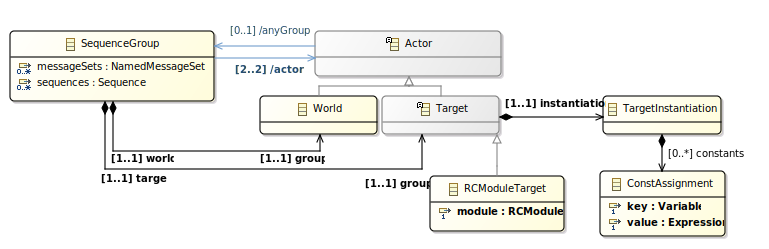
\includegraphics[width=\textwidth]{diagrams/Actors}
	\caption{Class diagram for the part of the \langname{} metamodel dealing with actors.}
	\label{fig:metamodel-actors}
\end{figure}

\Cref{fig:metamodel-actors} depicts the part of the metamodel concerning
actors.

\subsection{\mactor}

An \mactor{} is a named participant in a sequence.  The names can be used to
specify the source and recipient of communications in \mmessagespec{}s.
As mentioned in
\cref{sec:metamodel-sequences}, there are always two actors
attached to a sequence: a \mtarget{} (\cref{ssec:metamodel-actors-target})
and a \mworld{} (\cref{ssec:metamodel-actors-world}).

\subsection{\mtarget}\label{ssec:metamodel-actors-target}

A \mtarget{} references the part of a robotic system that serves as the focus
for a particular sequence diagram.  There is
presently one type of target, with more to appear later:

\begin{itemize}
\item
	a \mrcmoduletarget{} references a \mrcmodule.
\end{itemize}

All forms of \mtarget{} contain a \mtargetinstantiation{} (see below), which
is always applied to any use of that target; assertions may further instantiate
any constants left open by the target's \mtargetinstantiation.

\begin{lstlisting}[style=Example]
module AModule as M
// RCModuleTarget with implicit empty TargetInstantiation

module AModule
    with { SOME_CONSTANT set to 4, ANOTHER_CONSTANT set to 5 }
    as M
// RCModuleTarget with explicit TargetInstantiation
\end{lstlisting}

\subsection{\mtargetinstantiation}

A \mtargetinstantiation{} instantiates some or all of the constants in the
target's parametrisation.  It contains a list of key/value pairs where each key
is a RoboChart \mvariable{} corresponding to a constant, and each value is a
RoboChart \mexpression{} evaluated in an arbitrary \todo{check this} scope.

\begin{lstlisting}[style=Example]
{ SOME_CONSTANT set to 4, ANOTHER_CONSTANT set to 5 }
\end{lstlisting}

\subsection{\mworld}\label{ssec:metamodel-actors-world}

A \mworld{} is an \mactor{} that represents the `world' outside a sequence's
\mtarget.  \mworld s do not contain any data.

\begin{lstlisting}[style=Example]
world as W
\end{lstlisting}

%%% Local Variables:
%%% mode: latex
%%% TeX-master: "../robocert"
%%% End:


\section{Assertions}\label{sec:seq-metamodel-assertions}
%!TEX root=../robocert.tex
\begin{figure}
	\centering
	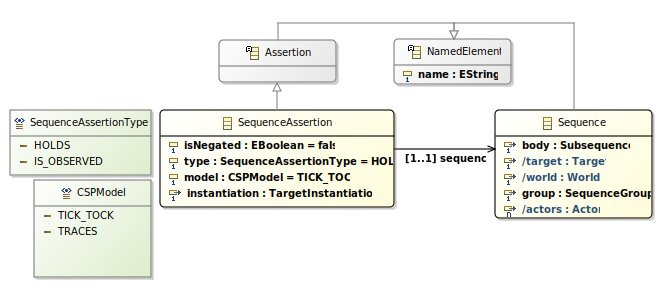
\includegraphics[width=0.7\textwidth]{diagrams/Assertions}
	\caption{Class diagram for the part of the \langname{} metamodel dealing with assertions.}
	\label{fig:metamodel-assertions}
\end{figure}

\Cref{fig:metamodel-assertions} depicts the part of the metamodel concerning
assertions.

\subsection{\massertion}

An \massertion{} is a named assertion statement.  Currently, there is
only one type of assertion: a \msequenceassertion{}.  \todo{This will change
when merging with the existing language, if not sooner.}

\subsection{\msequenceassertion}\label{ssec:metamodel-assertions-sequence}

A \msequenceassertion{} is an assertion about a particular \msequence{} with
respect to its \mtarget.  The \mtarget{} is modified by applying an
assertion-level \mtargetinstantiation, which may fix any constants not bound
by the sequence-level instantiation.  (The default is an empty instantiation,
meaning the target is exactly as specified at the sequence level.)

The specific sequence assertion type comes from the \msequenceassertiontype:
either `sequence holds on target' (refinement), or `sequence is observed on
target' (reverse refinement).  The assertion can be negated.  The choice of
\mcspmodel{} affects how the assertion is checked with CSP tools such as FDR
\todo{the models aren't actually used yet; everything is treated as untimed
traces refinement.  This will change.}

\begin{lstlisting}[style=Example]
assertion A: SequenceName holds           // positive 'holds' SequenceAssertion
assertion B: SequenceName does not hold   // negative 'holds' SequenceAssertion
assertion C: SequenceName is observed     // positive 'is observed' SequenceAssertion
assertion D: SequenceName is not observed // negative 'is observed' SequenceAssertion

assertion E: SequenceName holds with { CONSTANT set to 5 }
// example of SequenceAssertion with custom TargetInstantiation
\end{lstlisting}

%%% Local Variables:
%%% mode: latex
%%% TeX-master: "../robocert"
%%% End:


%%% Local Variables:
%%% mode: latex
%%% TeX-master: "../robocert"
%%% End:


\chapter{Semantics}
%!TEX root=./robocert.tex

% Target language colouration
\newcommand{\tlang}[1]{\textcolor{TColor}{\boxed{#1}}}
% Object language colouration (nested inside target language)
\newcommand{\olang}[1]{\boxed{\textcolor{ZedColor}{#1}}}

\newcommand{\tockcsp}{\emph{tock}-CSP}
\newcommand{\cspm}{CSP\(_\text{M}\)}

\newcommand{\defeq}{\mathbin{\overset{\text{def}}=}}
% CSP operators
\newcommand{\interrupt}{\mathbin{\triangle}}
\newcommand{\cspnsop}{\mathbin{\!:\!:\!}}
% CSP keywords/processes
\newcommand{\cspkw}[1]{\operatorname{\mathbf{#1}}}
\newcommand{\runproc}[1]{\cspkw{Run}\left(#1\right)}
\newcommand{\events}{\cspkw{Events}}

%
% Metasyntactic variables
%
\newcommand{\acontext}{c}
\newcommand{\anexpr}{e}
\newcommand{\avar}{v}
% Top-level
\newcommand{\apkg}{P}
\newcommand{\acsp}{f}
% Sequences
\newcommand{\aseq}{\sigma}
\newcommand{\asseq}{q}
% Steps
\newcommand{\astep}{s}
\newcommand{\anastep}{s_a}
\newcommand{\adeadline}{d}
\newcommand{\aloop}{l}
\newcommand{\agap}{g}
% Actions
\newcommand{\anaction}{a}
\newcommand{\anarrow}{\rho}
\newcommand{\await}{w}
% Messages
\newcommand{\amspec}{m}
\newcommand{\amsgset}{M}
\newcommand{\aumsgset}{\amsgset_{\universe}}
\newcommand{\anemsgset}{\amsgset_{e}}
\newcommand{\armsgset}{\amsgset_{r}}
\newcommand{\anevent}{\epsilon}
\newcommand{\anop}{o}
% - Arguments
\newcommand{\anarg}{x}
\newcommand{\anexprarg}{\anarg_\anexpr}
\newcommand{\arestarg}{\anarg_r}
\newcommand{\anarglist}{\mathbf{x}}
% Actors
\newcommand{\atarget}{t}
\newcommand{\aninst}{\phi}
\newcommand{\aworld}{w}
% Assertions
\newcommand{\anasst}{\alpha}
\newcommand{\asasst}{\alpha_s}
\newcommand{\amodel}{\mathcal{M}}

% External semantics
\newcommand{\exprsema}[2]{\sema{#1}{expr}_{(#2)}}

\newcommand{\sema}[2]{\llbracket #1 \rrbracket^{\mathsf{#2}}}
\newcommand{\pkgsema}[1]{\sema{#1}{pkg}}
\newcommand{\cspsema}[1]{\sema{#1}{csp}}
\newcommand{\stepsema}[1]{\sema{#1}{step}}
\newcommand{\gapsema}[2]{\sema{#1}{gap}_{(#2)}}
\newcommand{\actsema}[1]{\sema{#1}{act}}
\newcommand{\mspecsema}[2]{\sema{#1}{mspec}_{\text{#2}}}
\newcommand{\pmspecsema}[1]{\mspecsema{#1}{prefix}}
\newcommand{\emspecsema}[1]{\mspecsema{#1}{events}}
\newcommand{\arglistsema}[2]{\sema{#1}{args}_{(#2)}}
\newcommand{\loopsema}[1]{\sema{#1}{loop}}
\newcommand{\msgsetsema}[1]{\sema{#1}{mset}}
\newcommand{\seqsema}[1]{\sema{#1}{seq}}
\newcommand{\sseqsema}[1]{\sema{#1}{sseq}}
\newcommand{\asstsema}[1]{\sema{#1}{asst}}

\newcommand{\targetsema}[2]{\sema{#1}{target}_{(#2)}}

\newcommand{\funcname}[1]{\ensuremath{\mathsf{#1}}}
\newcommand{\eventsOf}[1]{\funcname{events}(#1)}
\newcommand{\seqnameOf}[1]{\funcname{seqName}(#1)}
\newcommand{\ctargetnameOf}[1]{\funcname{ctargetName}(#1)}
\newcommand{\otargetnameOf}[1]{\funcname{otargetName}(#1)}

\newcommand{\field}[2]{#1.\funcname{#2}}

This chapter formally captures the semantics of \langname{} in terms of its
target languages:

\begin{itemize}
\item
	\tockcsp~(\cref{sec:semantics-tockcsp});
\item
	\todo{PRISM};
\item
	\todo{Isabelle/UTP?}.
\end{itemize}

Each semantics captures \massertion s as the top-level definition, with all
objects reachable from the assertions translated in-line.  As a
consequence, we do not capture organisational details such as \mrapackage s,
or any distinction between references to objects and their definitions.

\section{How to read this section}

\begin{table}
  \centering

  \begin{tabular}{p{1.3em}p{9em}}
    \toprule
    \thead{Var.}
    & \thead{Type}
    \\
    \midrule
    \multicolumn{2}{l}{\tsubhead{\robochart{} imports}}
    \\
    \(\avar\) & \mvariable
    \\
    \(\anexpr\) & \mexpression
    \\
    \bottomrule
  \end{tabular}
  \begin{tabular}{p{1.3em}p{9em}}
    \toprule
    \thead{Var.}
    & \thead{Type}
    \\
    \midrule
    \multicolumn{2}{l}{\tsubhead{Packages (\cref{sec:metamodel-top})}}
    \\
    \(\apkg\) & \mrapackage
    \\
    \(\acsp\) & \mcspfragment
    \\
    \midrule
    \multicolumn{2}{l}{\tsubhead{Sequences (\cref{sec:metamodel-sequences})}}
    \\
    \(\aseq\) & \msequence
    \\
    \(\asseq\) & \msubsequence
    \\
    \midrule
    \multicolumn{2}{l}{\tsubhead{Steps (\cref{sec:metamodel-steps})}}
    \\
    \(\astep\) & \msequencestep
    \\
    \(\anastep\) & \mactionstep                 
    \\
    \(\agap\) & \msequencegap
    \\
    \(\adeadline\) & \mdeadlinestep
    \\
    \(\aloop\) & \mloopstep
    \\
    \midrule
    \multicolumn{2}{l}{\tsubhead{Actions (\cref{sec:metamodel-actions})}}
    \\
    \(\anaction\) & \msequenceaction
    \\
    \(\anarrow\) & \marrowaction
    \\
    \(\await\) & \mwaitaction
    \\
    \(\bot\) & \mfinalaction
    \\
    \\
    \bottomrule
  \end{tabular}
  \begin{tabular}{p{1.3em}p{9em}}
    \toprule
    \thead{Var.}
    & \thead{Type}
    \\
    \midrule
    \multicolumn{2}{l}{\tsubhead{Messages (\cref{sec:metamodel-messages})}}
    \\
    \(\amspec\) & \mmessagespec
    \\
    \(\amsgset\) & \mmessageset
    \\
    \(\aumsgset\) & \muniversemessageset
    \\
    \(\anemsgset\) & \mextensionalmessageset
    \\
    \(\armsgset\) & \mrefmessageset
    \\
    \midrule
    \multicolumn{2}{l}{\tsubhead{Arguments}}
    \\
    \(\anarg\) & \margument
    \\
    \(\anexprarg\) & \mexpressionargument
    \\
    \(\arestarg\) & \mrestargument
    \\
    \midrule
    \multicolumn{2}{l}{\tsubhead{Actors (\cref{sec:metamodel-actors})}}
    \\
    \(\atarget\) & \mtarget
    \\
    \(\aworld\) & \mworld
    \\
    \(\aninst\) & \mtargetinstantiation
    \\
    \midrule
    \multicolumn{2}{l}{\tsubhead{Assertions (\cref{sec:metamodel-assertions})}}
    \\
    \(\anasst\) & \massertion
    \\
    \(\asasst\) & \msequenceassertion
    \\
    \(\amodel\) & \mcspmodel	
    \\
    \bottomrule
  \end{tabular}
  
  \caption{Metasyntactic variables.}
  \label{tab:metasyntactic-variables}
\end{table}

The semantics treatments in this section take the form of rewrite rules from
the abstract syntax in \cref{cha:metamodel} to some object language (for
instance, \tockcsp).
For conciseness, we use a meta-language based on the Z notation.
We also use the following notational conventions:

\begin{itemize}
\item
	\(\sema{-}{name}\) denotes a main semantic rule;
\item
	\(\funcname{name}()\) denotes auxiliary semantic functions;
\item
	\(\field{x}{name}\) denotes a field of the metamodel object \(x\);
\item
	\tlang{\text{boxed shaded text}} denotes a construct from the object
	language; outside such text, or \tlang{\olang{\text{inside nested boxes}}},
	assume use of the meta-language.  For example, consider the \tockcsp{}
	construct:
	\[\tlang{
		\runproc{\olang{\gapsema{\field{\astep}{gap}}{\field{\astep}{action}}}}
		\interrupt \olang{\actsema{\field{\astep}{action}}}
	}\]
	Here, \(\runproc{}\) and \(\interrupt\) are part of \tockcsp, while
	\(\actsema{\field{\astep}{action}}\) is an semantic operation on the
	\langname{} metamodel.
\item
	variables in the meta-language have an implicit metamodel type
	corresponding to one of the metasyntactic variables in
	\cref{tab:metasyntactic-variables}.
\end{itemize}

\section{Dependencies on the \robochart{} semantics}

\newcommand{\targetProcess}[1]{\ensuremath{\funcname{targetProcess}\left(#1\right)}}
\newcommand{\targetParams}[1]{\ensuremath{\funcname{targetParams}\left(#1\right)}}
\newcommand{\constName}[1]{\ensuremath{\funcname{constName}\left(#1\right)}}

\todo{this may need to move to the \tockcsp{} section eventually}

Each semantics treatment in this section assumes the existence of a compatible
semantics over \robochart.  Specifically, we assume the following rules and
functions are available, or can be derived, from such a semantics:

\begin{itemize}
\item
	let \targetProcess{-} map a target to the parametric
	process exposed by the relevant \tockcsp{} semantics (for instance,
	we delegate to the \robochart{} semantics for the underlying
	\mrcmodule{} of a \mrcmoduletarget);
	\todo{doesn't account for the ID parameter in certain target
	processes};
\item
	let \targetParams{-} map a target to the sequence of
	constants in its parameterisation;
\item
	let \constName{-} map a constant to its name in the \robochart{}
	instantiations file;
\item
	let \(\exprsema{\anexpr}{\acontext}\) be the expression semantics of 
	\(\anexpr\) in the context \(\acontext\).  The expression semantics
	is external to this semantics, but is largely that of Z.
\end{itemize}

\section{\tockcsp{} semantics}\label{sec:semantics-tockcsp}
%!TEX root=../robocert.tex

This section introduces a \tockcsp{} semantics for \langname.

\section{Core language}\label{sec:semantics-tockcsp-core}

\section{Sequence notation}\label{sec:semantics-tockcsp-seq}
%!TEX root=robocert.tex

The \emph{sequence} notation of \langname{} provides a method of
defining the expected interactions between actors in a robotic model,
optionally with time constraints.  For instance, sequences may specify
how a \robochart{} module uses services offered by a robotic platform.
Sequences resemble UML sequence diagrams.

\chapter{Metamodel}\label{cha:metamodel}
\input{seq/metamodel}

\chapter{Textual syntax}\label{cha:textual}
\input{seq/textual}

\chapter{Graphical syntax}\label{cha:graphical}
\input{seq/graphical}

%%% Local Variables:
%%% mode: latex
%%% TeX-master: "robocert"
%%% End:


%%% Local Variables:
%%% mode: latex
%%% TeX-master: "../robocert"
%%% End:

%%% Local Variables:
%%% mode: latex
%%% TeX-master: "robocert"
%%% End:


\end{document}